\clearpage
\subsection{Pass by Value and Pass by Reference} % (fold)
\label{sub:pass_by_value_and_pass_by_reference}

There are actually two ways that values can be passed to Parameters. This relates back to the fact that Variables have two aspects: the Value within the Variable, and the Variable itself. These two means of passing parameters allow you to either pass a value, or pass a Variable.

\begin{figure}[h]
   \centering
   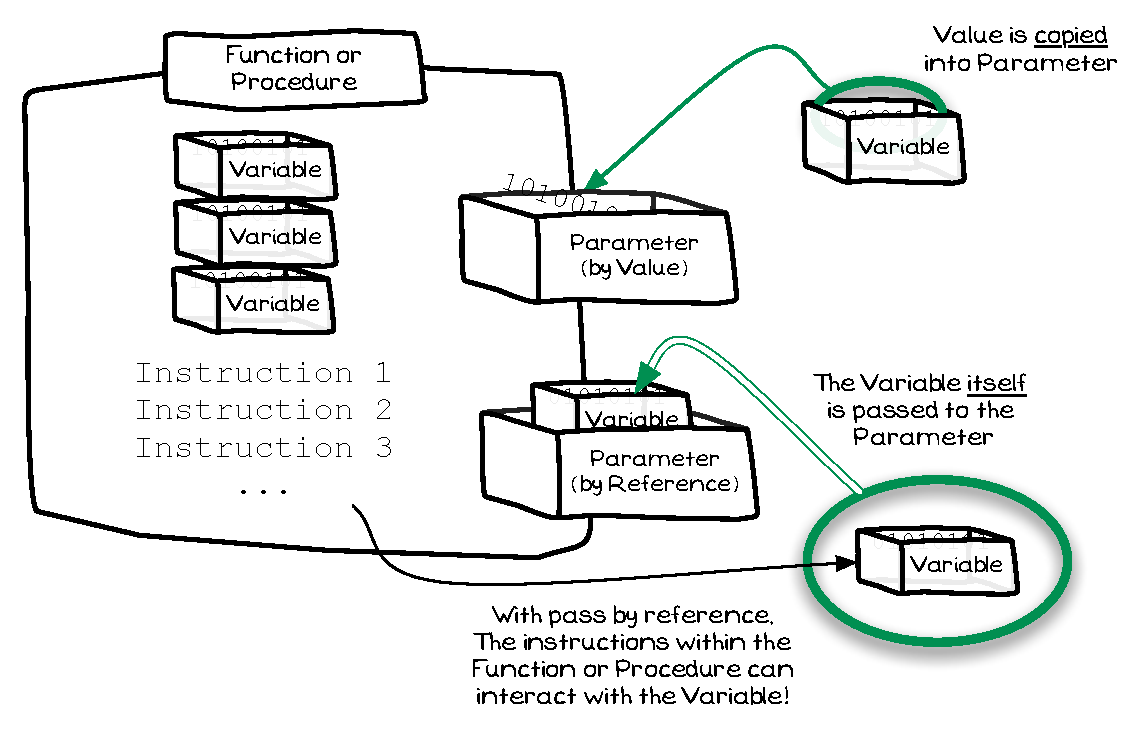
\includegraphics[width=\textwidth]{./topics/storing-using-data/diagrams/ByValByRef} 
   \caption{Parameters can accept data by reference or by value}
   \label{fig:parameters-parameters}
\end{figure}

\mynote{
\begin{itemize}
  \item Pass by Reference and Pass by Value are \textbf{terms} that explain how data is passed to a Parameter.
  \item Most parameters are passed by value.
  \item Pass by value copies the value to the parameter. This means pass by value can work with any Expression.
  \item Pass by reference allows you to pass the Variable itself to the parameter.
  \item The main use for pass by reference is to allow the Procedure or Function to store a value in the Variable passed to the parameter.
  \item It is called pass by reference due to the way it is implemented, with the parameter receiving a reference to the Variable. Section \ref{sec:using_these_concepts_storing_using_data} will cover this in more detail, conceptually the Variable itself is passed to the Parameter.
\end{itemize}
}

% subsection pass_by_reference (end)